\section{Introduction}
\subsection{Overview}
%
The choice for our game fell on cloning the open-source game \emph{Frozen-Bubble}~\cite{website:frozenbubble}. 
%The reasons 
%for this are three-fold:
%
%\begin{itemize}
%  \item We looked for a game that we like to play alot ourselves
%  \item The game should not be too ressource hungry, as we were planning
%    on running it on the OLPC-XO
%  \item Not having any good graphic designers in our team, we wanted an
%    open game to be able to re-use images and quickly come up with something
%    good looking
%\end{itemize}
%
Within the game, the user controls a small canon, shooting bubbles and tries to 
hit other bubbles in order to create groups of 3 or more bubbles of the same color. 
Whenever this is accomplished these bubbles go away and the player gains points. 
For a larger number of balls the 
player is awarded exponentially more points, so the goal is to clear out large numbers 
of balls at once by building chains and removing balls near the top of the chain.
In single player mode, the game goes on as long as the balls do not reach the bottom 
of the stage, much like popular arcade games as, for example, Tetris or Puyo-Puyo.
In multiplayer mode players compete and try to delay filling their playfield 
as long as possible.
%
\subsection{The Original}
The original Frozen-Bubble was written in Perl using the \emph{Simple Direct Media Layer} (SDL)
for graphics and sound. It was developed within three months and had its first official 
release at the end of january, 2002. While initially it only ran on GNU/Linux it has since
been ported to other operating systems supported by SDL, thanks to being licensed under the GPLv2.
It also runs on the Symbian\trademark
S60 platform, the Palm\registered operating system and as Java\trademark applet in the 
browser\footnote{Symbian is a trademark of Symbian Foundation, Palm is a registered trademark 
of Palm, Inc. and Java is a trademark of Sun Microsystems}. 

\begin{wrapfigure}{r}{0.5\textwidth}
\vspace{-2em}
  \begin{center}
    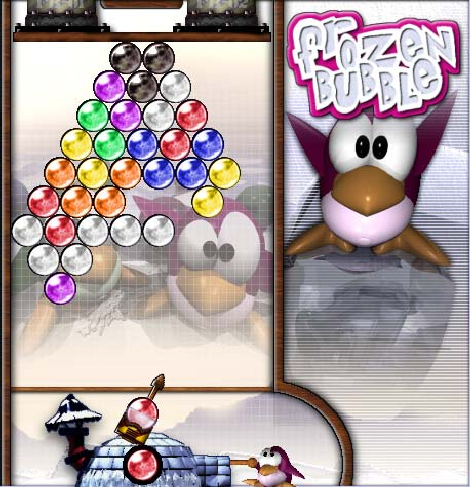
\includegraphics[width=0.44\textwidth]{images/screenshot1}
  \end{center}
  \vspace{-1em}
  \caption{A view of the original Frozen Bubble with the 2.0 theme}
\vspace{-2em}
\end{wrapfigure}

The original game features a single player mode with multiplet levelsets. Each level 
of a level set defines an initial playfield layout and
a level finishes when the player manages to remove all balls 
from the playfield.\\
Additionally, the original game also has a multiplayer mode for two players 
locally and up to five players over the network. Here, the goal is to clear the balls 
faster and more efficiently than your opponents, and clearing a great number of balls 
is rewarded by adding ``penalty balls'' to the opponents' playfields.
%
\subsection{The Clone}
Our clone of the Frozen-Bubble game keeps the name in consensus with the original developers.
We have also aquired the permissions of the original artist to release his graphics 
together with our code under the MIT license.
The single player experience has been changed as stated above to relief us from the need 
to have to supply levelsets with the game.\\
We have not implemented a networked multiplayer mode, however, playing locally against 
a human opponent works to a fair extent as in the original.

However, our interpretation introduces some slight changes to the gaming experience.
Most notably we support ``realistic'' collision instead of a hex-field for the balls, which
makes playing a lot more challenging. In the visual side, we support more flexible theming.
In the original that has not been a goal, so ``themes'' are limited 
to replacing PNG graphics.
%
\subsection{Design Goals}
In order to achieve a pleasant and cleanly written FrozenBubble clone, we specified certain design goals.
A goal we set for ourselves very early was themeability, e.g. the ability to modify and adjust certain visual and logical aspects of the game (for example ball images or cannon positions). This demands an efficient and maintainable theme management system, as lots of pictures and data need to be processed.
As previously stated, another important aspect of our clone is ''realistic'' collision between objects. To achieve this, an algorithm other than simply looping through all objects present to counter the hardware limitations of the OLPC-XO.
Lastly, we want our game to support multiplayer functionality. Given the time needed to implement networking, we decided to focus on a local multiplayer modes.
%
\subsection{Outline}
In this paper, we will present our game design and shed some light on the decisions 
it is based on. We will begin with an introduction to our system architecture and 
gradually expand that to include the whole system structure.\\
Finally we will outline our development plan and process and elaborate on the 
future of our project, licensing issues and the like.
%
